%%%%%%%%%%%%%%%%%%%%%%%%%%%%%%%%%%%%%%%%%%%%%%%%%%%%%%%%%%%%%%%%%%%%%%%%%%%%%%%%
\section{Cosine of Normalised Gradients}\label{sec:singl_img_cosine_normalised_gradients}
%%%%%%%%%%%%%%%%%%%%%%%%%%%%%%%%%%%%%%%%%%%%%%%%%%%%%%%%%%%%%%%%%%%%%%%%%%%%%%%%
In this section, we describe the concept of the cosine of normalised gradients
and specify how they represent a robust measure of similarity. In this work, we
consider a similarity measure to be robust if it suppresses the contribution of
comparisons between image areas that are unrelated. More specifically, we seek a
measure that, when given two images that are visually dissimilar, will calculate
zero correlation between them. For example, consider
\cref{fig:tumour_examples} which shows cross sections of a brain containing a 
tumour. When registering this corrupted image with an image of a healthy brain, 
the ideal registration would not be biased by the presence of the tumour, as it 
does not share relevant anatomical structures with the healthy brain.
To this end, \citet{RefWorks:68,RefWorks:6} proposed the
cosine of orientation differences between two images, which we describe in
detail below.
%%%%%%%%%%%%%%%%%%%%%%%%%%%%%%%%%%%%%%%%%%%%%%%%%%%%%%%%%%%%%%%%%%%%%%%%%%%%%%%%
\subsection{Cosine Similarity in 2D}\label{subsec:cosine_2d}
%%%%%%%%%%%%%%%%%%%%%%%%%%%%%%%%%%%%%%%%%%%%%%%%%%%%%%%%%%%%%%%%%%%%%%%%%%%%%%%%
%TODO: Fix figures
%%%%%%%%%%%%%%%%%%%%%%%%%%%%%%%%%%%%%%%%
% \begin{figure*}
%     \centering
%     \hspace*{\fill}
%     \begin{subfigure}[t]{0.33\textwidth}
%         \centering
%         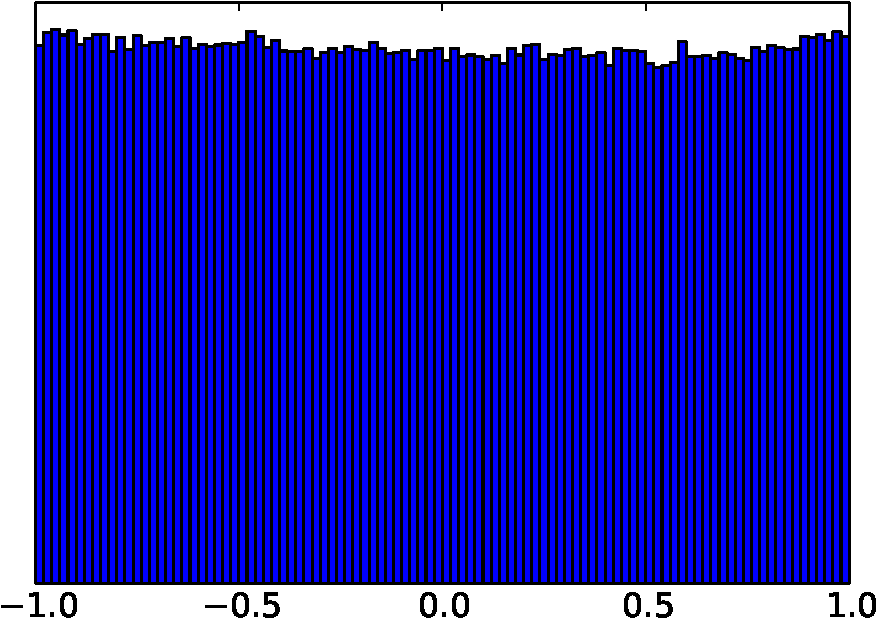
\includegraphics[width=\textwidth]{images/distributions/inner_product_tumour-crop}
%         \caption{$\cos{\sigma}$ tumour area}\label{subfig:inner_product_tumour}
%     \end{subfigure} \hfill
%     \begin{subfigure}[t]{0.32\textwidth}
%         \centering
%         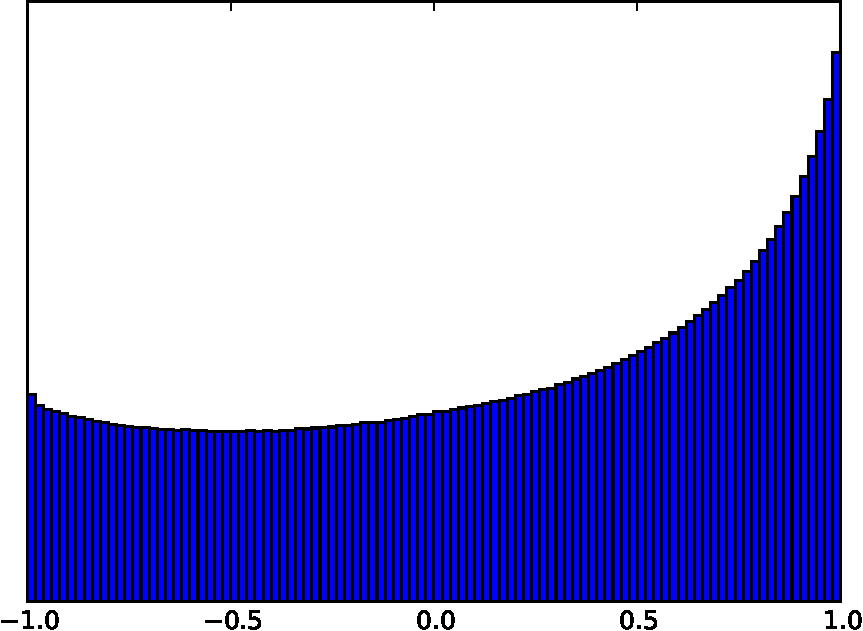
\includegraphics[width=\textwidth]{images/distributions/inner_product_all-crop}
%         \caption{$\cos{\sigma}$ entire image}\label{subfig:inner_product_all}
%     \end{subfigure} \hfill
%     \begin{subfigure}[t]{0.33\textwidth}
%         \centering
%         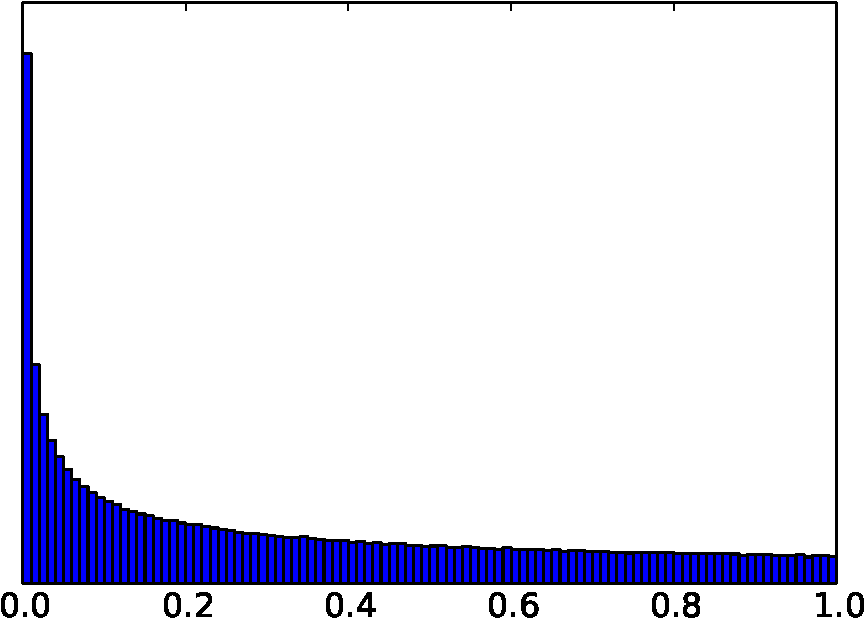
\includegraphics[width=\textwidth]{images/distributions/inner_product_squared_tumour-crop}
%         \caption{$\cos^{2}{\sigma}$ tumour area}\label{subfig:inner_product_squared_tumour}
%     \end{subfigure}
%     \hspace*{\fill}
%     \caption{The distributions of $\cos{\sigma}$ and $\cos^2{\sigma}$ averaged 
%              over 10 subjects from the BraTS simulated images. The images were
%              registered using a rigid transformation prior to computation and
%              only the tumour areas were sampled. (a) shows the distribution of
%              $\cos{\sigma}$ in the simulated tumour region. (b) shows the
%              distribution of $\cos{\sigma}$ over the entire image. (c) shows the
%              distribution of $\cos^2{\sigma}$ proposed
%              in~\cite{haber2006intensity} in the simulated tumour region}
% \label{fig:inner_product_distributions}
% \end{figure*}
%%%%%%%%%%%%%%%%%%%%%%%%%%%%%%%%%%%%%%%%
Assuming we are given two 2D images, denoted as $I_i \; i \in \{1,2\}$, we
define $G_{i,x} = \bb{F}_x \ast I_i$ and $G_{i,y} = \bb{F}_y \ast I_i$
as the gradients obtained by convolving $I_i$ with differentiation approximation
filters $\bb{F}_x$ and $\bb{F}_y$ respectively. We denote the
lexicographical vectorisation of $G_{i,x}$ as $\bb{g}_{i,x}$ and define an
index $k$ into the vector, $\bb{g}_{i,x}(k)$. We define an identical vector
for $G_{i,y}$ as $\bb{g}_{i,y}$. We also define $\bb{g}_{i}(k)$ as the
vector formed by concatenating the $x$ and $y$ gradients together. Trivially, we
can define the normalised gradient as $\bb{\tilde{g}}_{i}(k) =
\frac{\bb{g}_{i}(k)}{\norm{\bb{g}_{i}(k)}}$ where
$\norm{\bb{g}_{i}(k)} = {\sqrt{g_{i,x}(k)}^2 + {g_{i,y}(k)}^2}$.  We also define
similar vectors for the $x$ and $y$ components separately, with
$\bb{\tilde{g}}_{i,x}$ being the $x$ components concatenated in
lexicographical ordering and $\bb{\tilde{g}}_{i,y}$ being the $y$ components.
Finally, $\bb{\tilde{g}}_{i}$ is the vector of concatenated normalised
gradients for image $I_i$.

Given the normalised gradients, it is simple to parametrise them within a polar
coordinate system with radius $r_i(k) = \lVert \bb{\tilde{g}}_{i}(k) \rVert
= 1$, orientation $\phi_i(k) =
\arctan{\frac{\tilde{g}_{i,y}(k)}{\tilde{g}_{i,x}(k)}}$ and pole at the origin.
Given orientations from two dissimilar images, it is reasonable to assume that
difference between the orientations, $\Delta \phi(k) = \phi_1(k) - \phi_2(k)$,
can take any angle between $[0, 2\pi)$. Intuitively, this implies that selecting
two pixels from dissimilar images is unlikely to yield any correlation between
the images. In~\cite{RefWorks:6}, it was experimentally verified that the
orientation differences follow a uniform distribution, $\Delta \phi(k) \sim U(0,
2\pi)$. The fact that the orientation differences follows a uniform distribution
is unsurprising under the assumption that the two images have absolutely no
correlation. However, the expectation of the cosine of the uniform distribution
is zero, which is a powerful property that can be exploited for image
registration. It is powerful because it means that the expected overall
contribution of uncorrelated areas to any cost function will be zero, meaning
the uncorrelated areas do not affect the result of the registration.

Formally, we assume $\Delta \phi(k)$ is a stationary random process $y(t)$ with
index $t \triangleq k \in \mathcal{R}^2$, where $\forall t \sim U(0, 2\pi)$. We
define the random process $z(t) = \cos{y(t)}$ and thus $\forall t$ random
variable $Z = z(t)$ has mean value $E\{Z\} = 0$. In fact, by assuming mean
ergodicity, we find that
%%%%%%%%%%%%%%%%%%%%%%%%%%%%%%%%%%%%%%%%%%%%%%%%%%%%%%%%%%%%%%%%%%%%%%%%%
\begin{equation}\label{eq:cosine_integral}
    E\{Z\} \propto \int z(t) dt \equiv \int_{\mathcal{R}^2} \cos[\Delta \phi(k)] dk = 0
\end{equation}
%%%%%%%%%%%%%%%%%%%%%%%%%%%%%%%%%%%%%%%%%%%%%%%%%%%%%%%%%%%%%%%%%%%%%%%%%
This is an important property for a similarity measure to be robust against
occlusions. Since occlusions do not provide useful information for alignment,
ideally they would be ignored. However, manual segmentation of occluded areas is
time consuming and prone to error. Therefore, an ideal robust similarity measure
would be able to automatically identify regions of the image that are occluding
the true object of interest. Under the previous definition of robustness, the
cosine similarity naturally represents a robust similarity measure as it
automatically suppresses the contribution of outliers.

Given an image warping function with parameters $\bb{p}$, maximising the sum
of the cosine of orientation differences provides the robust similarity measure:
%%%%%%%%%%%%%%%%%%%%%%%%%%%%%%%%%%%%%%%%%%%%%%%%%%%%%%%%%%%%%%%%%%%%%%%%%
\begin{equation}\label{eq:2d_similarity_measure}
    q = \sum_k \cos \left(\Delta \phi(k)[\bb{p}]\right)
\end{equation}
%%%%%%%%%%%%%%%%%%%%%%%%%%%%%%%%%%%%%%%%%%%%%%%%%%%%%%%%%%%%%%%%%%%%%%%%%
For more details of the specifics of optimising (\ref{eq:2d_similarity_measure})
for image alignment, we refer the reader to~\cite{RefWorks:6}.
%%%%%%%%%%%%%%%%%%%%%%%%%%%%%%%%%%%%%%%%%%%%%%%%%%%%%%%%%%%%%%%%%%%%%%%%%%%%%%%%
\subsection{Cosine Similarity in 3D}\label{subsec:cosine_3d}
%%%%%%%%%%%%%%%%%%%%%%%%%%%%%%%%%%%%%%%%%%%%%%%%%%%%%%%%%%%%%%%%%%%%%%%%%%%%%%%%
We make very similar assumptions for 3D images as we did in
\cref{subsec:cosine_2d} for 2D images. We simply extend the previous
notation by including the gradient of the $z$-axis, denoted as $G_{i,z} = \bb{F}_z \ast I_i$. 
We also redefine the normalised gradient as
$\bb{\tilde{g}}_{i}(k) = \frac{\bb{g}_{i}(k)}{\norm{\bb{g}_{i}(k)}}$
where $\norm{\bb{g}_{i}(k)} = {\sqrt{g_{i,x}(k)}^2 + {g_{i,y}(k)}^2 +
{g_{i,z}(k)}^2}$ and $\bb{g}_{i}(k)$ is defined as the vector formed by
concatenating the $x$, $y$ and $z$ gradients together.

Measuring the angular distance between vectors in 3D is more complex than in 2D,
due to the extra degree of freedom. In the following sections, we describe two
different measures that can be used to calculate similarities between vectors
within 3D images, the spherical coordinates and the inner product. In the
previous section, we described in detail how properties of the cosine of a
uniform distribution can be exploited to form a robust measure of similarity.
The most important property was that uncorrelated areas such as occlusions
should have no impact registration. This was formalised as the expectation of
the sum of the uncorrelated elements should be zero. In the case of input to the
cosine function, a given distribution must simply be symmetric over the positive
and negative span of outputs of the cosine. When symmetric over the positive and
negative outputs, the expectation of the cosine function is zero. In fact, we
can relax the definition of a measure being robust to outliers by stating that
we desire a measure whereby the expectation of the measure over image areas that
are uncorrelated is zero.

In practise, when comparing two images where one image contains occlusions,
there will be regions that are correlated and then the occluded region that is
uncorrelated. In this case, the total distribution of all pixels will be
described by a mixture model of the occluded and non-occluded regions. We desire
that the distribution of the uncorrelated areas has an expectation of zero and
thus will not affect the optimisation of the similarity measure.

In \cref{subsubsec:cosine_spherical} and
\cref{subsubsec:cosine_inner_product} we describe two measures of angular
difference between 3D images. We investigate the distribution of these angular
measures when combined with the cosine function and motivate that they are both
suitable for use as a similarity measure between real 3D images.
%%%%%%%%%%%%%%%%%%%%%%%%%%%%%%%%%%%%%%%%%%%%%%%%%%%%%%%%%%%%%%%%%%%%%%%%%%%%%%%%
\subsubsection{Spherical Coordinates}\label{subsubsec:cosine_spherical}
%%%%%%%%%%%%%%%%%%%%%%%%%%%%%%%%%%%%%%%%%%%%%%%%%%%%%%%%%%%%%%%%%%%%%%%%%%%%%%%%
In 2D, a natural parametrisation of the angle between the two gradient vectors
is the polar coordinate system. In 3D, we have three gradient vectors and thus
require two angles to describe their orientation. Unlike in 2D, where the
vectors lie on the unit circle, in 3D the vectors lie on the surface of a unit
sphere. Therefore, it is possible to parametrise the vectors in terms of the
spherical coordinate system, which is described by two angles: the azimuth angle
$\phi$ with range $[0, 2\pi)$ and the elevation angle $\theta$ with range
$[0, \pi]$. Given the normalised gradients as vectors with Cartesian
coordinates, we can calculate the spherical angles as follows:
%%%%%%%%%%%%%%%%%%%%%%%%%%%%%%%%%%%%%%%%%%%%%%%%%%%%%%%%%%%%%%%%%%%%%%%%%
\begin{equation}\label{eq:cartesian_to_spherical}
    \begin{aligned}
        r_i(k)      &= \lVert \bb{\tilde{g}}_{i}(k) \rVert = 1            \\
        \phi_i(k)   &= \arctan{\frac{\tilde{g}_{i,y}(k)}{\tilde{g}_{i,x}(k)}} \\
        \theta_i(k) &= \arccos{\tilde{g}_{i,z}(k)}
    \end{aligned}
\end{equation}
%%%%%%%%%%%%%%%%%%%%%%%%%%%%%%%%%%%%%%%%%%%%%%%%%%%%%%%%%%%%%%%%%%%%%%%%%
An illustration of the spherical coordinate system, as used in this paper, is
given in \cref{fig:spherical_coordinates}.

Our proposal is to combine the spherical coordinates with the cosine function in
order to provide a robust similarity measure. Similar to the 2D case,, we
propose the cosine of azimuth differences, $\Delta \phi = \phi_1 - \phi_2$, and
the cosine of elevation differences, $\Delta \theta = \theta_1 - \theta_2$, as a
combined similarity measures. Given a 3D image warping function with parameters
$\bb{p}$, the spherical coordinates form a similarity measure as follows:
%%%%%%%%%%%%%%%%%%%%%%%%%%%%%%%%%%%%%%%%%%%%%%%%%%%%%%%%%%%%%%%%%%%%%%%%%
\begin{equation}\label{eq:spherical_similarity_measure}
    q = \sum_k \cos \left(\Delta \phi(k)[\bb{p}]\right) + \sum_k \cos \left(\Delta \theta(k)[\bb{p}]\right)
\end{equation}
%%%%%%%%%%%%%%%%%%%%%%%%%%%%%%%%%%%%%%%%%%%%%%%%%%%%%%%%%%%%%%%%%%%%%%%%%
Optimisation of (\ref{eq:2d_similarity_measure}) is described in detail in
\cref{sec:robust_lk}.

Experimentally, we verified that $\Delta \phi$ approximates a symmetric
distribution for simulated tumour data taken from the Multimodal Brain Tumor
Image Segmentation (BraTS) challenge, as shown in
\cref{fig:phi_distribution}. \cref{subfig:phi_tumour} shows the
distribution of $\Delta \phi$ between the tumour area circled in yellow in
\cref{fig:tumour_examples} and a healthy brain. The images were registered
using a rigid transformation before $\Delta \phi$ was computed.  The azimuth
angle is analogous to the angle studied in~\cite{RefWorks:68} and follows the
same uniform distribution, $\Delta \phi \sim U(0, 2\pi)$.

When the entire region of the rigidly registered brain images is considered, we
find that the distribution of $\Delta \phi$ is clearly a mixture of two separate
models, one for the occluded area and one for the rigidly registered area.
\cref{subfig:phi_all} shows the distribution of $\Delta \phi$ calculated
over the entire image region of each image and a Laplacian distribution that
best fits the data. Thus, our experimental evidence suggests that the total
distribution of $\Delta \phi$ over the entire image region is a mixture model
between a uniform distribution and a Laplacian distribution with approximately
zero mean.
% The elevation angle, however, appears to have a very interesting and novel distribution. \cref{fig:delta_theta} shows that the distribution of $\Delta \theta$ approximates a Von Mises distribution. Therefore, given the range of $\Delta \theta$, \cref{fig:sin_delta_theta} shows that the correct robust function for $\Delta \theta$ is in fact the sine function, $\sin{\Delta \theta}$. Although \cref{fig:sin_delta_theta} has heavy tails at $-1$ and $1$, the distribution is symmetric and has been experimentally verified to have an expected value of $0$. However, since $\Delta \theta$ is symmetric over the range of the sine function and since (\ref{eq:cosine_integral}) holds analogously for the sine function, then $\sin{\Delta \theta}$ represents a robust measure of similarity.
%%%%%%%%%%%%%%%%%%%%%%%%%%%%%%%%%%%%%%%%
% \begin{figure}
%     \centering
%     \begin{subfigure}{0.32\columnwidth}
%         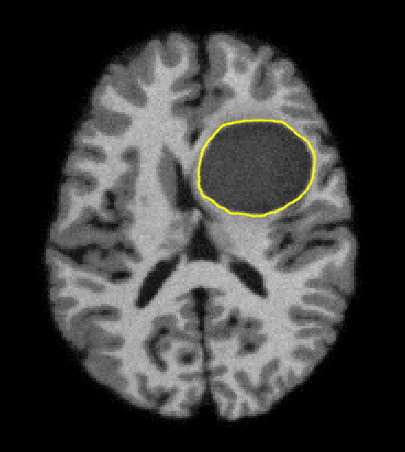
\includegraphics[width=\textwidth]{images/tumour_example_axial}
%     \end{subfigure}
%     \begin{subfigure}{0.32\columnwidth}
%         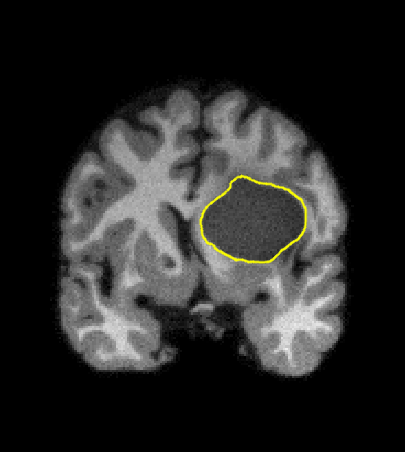
\includegraphics[width=\textwidth]{images/tumour_example_coronal}
%     \end{subfigure}
%     \begin{subfigure}{0.32\columnwidth}
%         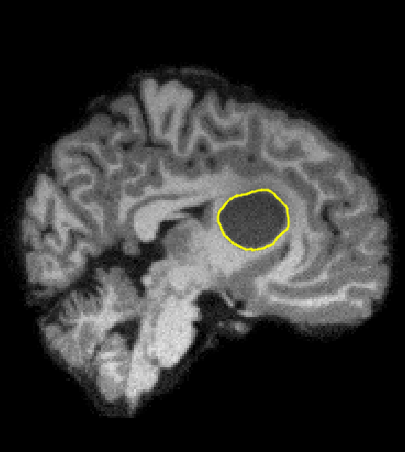
\includegraphics[width=\textwidth]{images/tumour_example_sagital}
%     \end{subfigure}
%     \caption{Example images of a T1-weighted brain containing a tumour area. 
%              The tumour areas are outlined in yellow in each image.
%              Left: Axial View. Middle: Coronal View. Right: Sagital View.}
% \label{fig:tumour_examples}
% \end{figure}
%%%%%%%%%%%%%%%%%%%%%%%%%%%%%%%%%%%%%%%%
% %%%%%%%%%%%%%%%%%%%%%%%%%%%%%%%%%%%%%%%%
% \begin{figure}
%     \centering
%     \begin{subfigure}{0.47\columnwidth}
%         \includegraphics[width=\textwidth]{images/tumour_example_3d}
%     \end{subfigure}
%     \begin{subfigure}{0.47\columnwidth}
%         \includegraphics[width=\textwidth]{images/healthy_example_3d}
%     \end{subfigure}
%     \caption{Example images of T1-weighted brain images of a single individual.
%              Left: Simulated tumour. 
%              Right: The original healthy brain.}
% \label{fig:3d_tumour_example}
% \end{figure}
% %%%%%%%%%%%%%%%%%%%%%%%%%%%%%%%%%%%%%%%%
%%%%%%%%%%%%%%%%%%%%%%%%%%%%%%%%%%%%%%%%%%%%%%%%%%%%%%%%%%%%%%%%%%%%%%%%%%%%%%%%
\subsubsection{Inner Product}\label{subsubsec:cosine_inner_product}
%%%%%%%%%%%%%%%%%%%%%%%%%%%%%%%%%%%%%%%%%%%%%%%%%%%%%%%%%%%%%%%%%%%%%%%%%%%%%%%%
A more general angular measure between two vectors is the inner product. Unlike
in~\cite{RefWorks:6} or \cref{subsubsec:cosine_spherical}, the inner
product is a single angle and not the difference between two angles.
Practically, the inner product measures the projection error between two vectors
and is defined as:
%%%%%%%%%%%%%%%%%%%%%%%%%%%%%%%%%%%%%%%%%%%%%%%%%%%%%%%%%%%%%%%%%%%%%%%%%
\begin{equation}\label{eq:inner_product}
    \cos{\sigma} = \bb{\tilde{g}}_{1}^{\top} \bb{\tilde{g}}_{2}
\end{equation}
%%%%%%%%%%%%%%%%%%%%%%%%%%%%%%%%%%%%%%%%%%%%%%%%%%%%%%%%%%%%%%%%%%%%%%%%%
In~\cite{RefWorks:68}, the authors reasonably propose that the angle between the
gradients of dissimilar images can take any value in $[0, 2\pi)$ with equal
probability. Similarly, the relationship between the gradient vectors of two
dissimilar 3D images could feasibly be in any direction with equal probability.
Therefore, the distribution of inner products between two unrelated vectors can
take the values $[-1, 1]$ with equal probability. Due to the expected range of
inner product values, we would expect that $\cos{\sigma}$ follows a uniform
distribution, $\cos{\sigma} \sim U(-1, 1)$. Note that this is a different
assumption to that made in~\cite{RefWorks:68}, which assumes that the
\textit{azimuth angle itself}, $\Delta \phi$, follows a uniform distribution.
However, it is merely sufficient that the total sum of values from the
dissimilar vectors is zero. Therefore, since $E\{U(-1, 1)\} = 0$, the inner
product of normalised gradients satisfies our definition of being robust to
outliers. In \cref{subfig:inner_product_tumour}, we show that this
assumption holds for the simulated tumour data taken from the BraTS challenge.

When the entire region of the rigidly registered brain images is considered, we
find that the distribution of $\cos{\sigma}$ is clearly a mixture of two
separate models, one for the occluded area and one for the rigidly registered
area. \cref{subfig:inner_product_all} shows the distribution of
$\cos{\sigma}$ calculated over the entire image region. In this case, the
distribution of the inner product appears to be a mixture model between a
uniform distribution and a zero mean Laplacian distribution. However, due to the
ambiguity in the inner product in terms of orientation, the angle of the inner
product is only defined in the range $[0, \pi]$ and thus only the positive tail
of the Laplacian appears.

In \cref{subfig:inner_product_squared_tumour} we also show the
distribution of the similarity measure proposed by \citet{haber2006intensity}. 
In~\cite{haber2006intensity}, the authors propose the inner product as a
similarity measure, which looks very similar to the measure we proposed in
\cref{eq:inner_product}. However, \citet{haber2006intensity} maximise the square of the
inner product using a least squares Gauss-Newton optimisation. As we have shown,
the inner product is related to the cosine between the vectors.
\citet{haber2006intensity} proposed the inner product squared as
a similarity, which is equivalent to the \textit{square of the cosine}. As we
can see in \cref{subfig:inner_product_squared_tumour}, the cosine squared
does not represent a symmetric distribution and therefore is not a robust
similarity measure by our definition.
%%%%%%%%%%%%%%%%%%%%%%%%%%%%%%%%%%%%%%%%
% \begin{figure}
%     \centering
%     \hspace*{\fill}
%     \begin{subfigure}[b]{0.46\columnwidth}
%     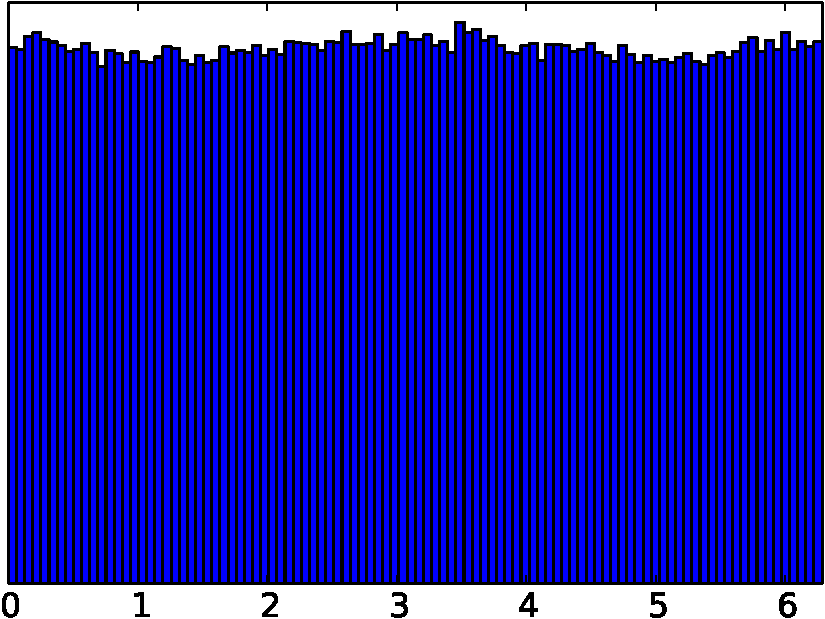
\includegraphics[width=\textwidth]{images/distributions/delta_phi_tumour-crop}
%     \caption{}\label{subfig:phi_tumour}
%     \end{subfigure}
%     \hfill
%     \begin{subfigure}[b]{0.45\columnwidth}
%     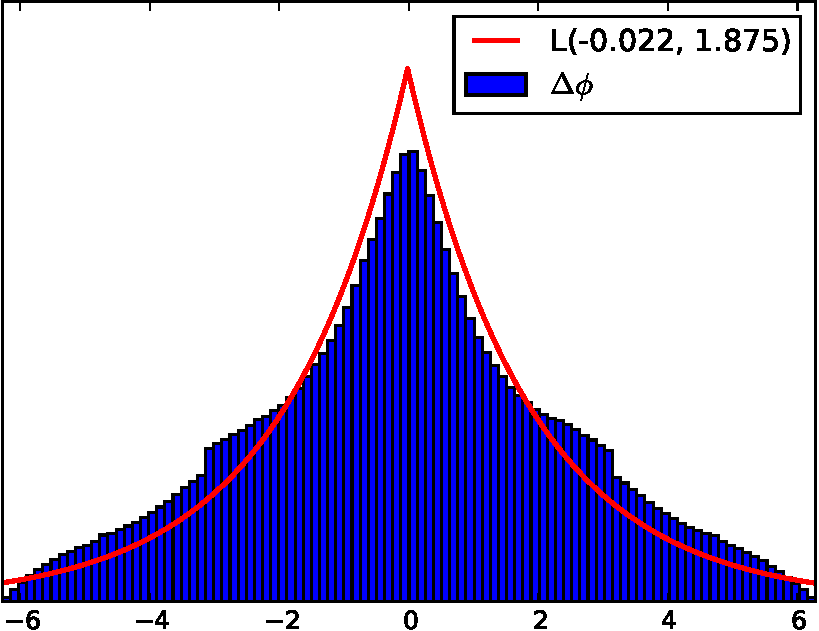
\includegraphics[width=\textwidth]{images/distributions/delta_phi_all_laplacian-crop}
%     \caption{}\label{subfig:phi_all}
%     \end{subfigure}
%     \hspace*{\fill}
%     \caption{The mean distribution of $\Delta \phi$ of the BraTS simulated images. 
%              The images were registered using a
%              rigid transformation and only the tumour
%              areas were sampled. (a) the distribution of $\Delta \phi$
%              in the simulated tumour region. (b) the distribution of
%              $\Delta \phi$ over the entire image. It also shows the
%              Laplacian distribution that best fits the data.}
% \label{fig:phi_distribution}
% \end{figure}
%%%%%%%%%%%%%%%%%%%%%%%%%%%%%%%%%%%%%%%%
%%%%%%%%%%%%%%%%%%%%%%%%%%%%%%%%%%%%%%%%%%%%%%%%%%%%%%%%%%%%%%%%%%%%%%%%%%%%%%%%
